% Build with XeLaTeX twice. Main talk: 12 slides; 3 optional appendix slides.
\documentclass[aspectratio=169,11pt]{beamer}
\usepackage{fontspec,polyglossia}
\setdefaultlanguage{russian}\setotherlanguage{english}
\setsansfont{DejaVu Sans}\setmainfont{DejaVu Sans}
\setmonofont{DejaVu Sans Mono}[Scale=0.78]
\newfontfamily\cyrillicfont{DejaVu Sans}
\newfontfamily\cyrillicfontsf{DejaVu Sans}
\newfontfamily\cyrillicfonttt{DejaVu Sans Mono}[Scale=0.78]
\usepackage{amsmath,amssymb,booktabs,array,graphicx,tikz,listings}
\usetikzlibrary{arrows.meta,positioning,calc}
\definecolor{Navy}{HTML}{12364A}\definecolor{Teal}{HTML}{087E80}
\definecolor{Amber}{HTML}{AD6020}\definecolor{Mist}{HTML}{EAF4F3}\definecolor{Pale}{HTML}{F2F5F8}
\setbeamercolor{normal text}{fg=Navy,bg=white}\setbeamercolor{structure}{fg=Teal}
\setbeamercolor{frametitle}{fg=Navy}\setbeamercolor{block title}{fg=white,bg=Teal}
\setbeamercolor{block body}{fg=Navy,bg=Mist}\setbeamercolor{alerted text}{fg=Amber}
\setbeamerfont{frametitle}{size=\Large,series=\bfseries}
\setbeamersize{text margin left=8mm,text margin right=8mm}
\setbeamertemplate{navigation symbols}{}\setbeamertemplate{itemize items}[circle]
\setbeamertemplate{footline}{\hspace{8mm}\raisebox{2mm}{\scriptsize\color{Teal}episynth / prequential PoC}\hfill\raisebox{2mm}{\scriptsize\insertframenumber\,/\,\inserttotalframenumber}\hspace{8mm}}
\setbeamertemplate{frametitle}{\vspace{3mm}\insertframetitle\par\vspace{1mm}{\color{Teal}\rule{\textwidth}{0.7pt}}}
\setlength{\emergencystretch}{1.5em}
\lstset{language=Python,basicstyle=\ttfamily\footnotesize,keywordstyle=\color{Teal}\bfseries,commentstyle=\color{gray},stringstyle=\color{Amber},showstringspaces=false,breaklines=true,columns=fullflexible,keepspaces=true,backgroundcolor=\color{Pale},frame=single,rulecolor=\color{Pale},xleftmargin=2mm,xrightmargin=2mm}
\newcommand{\code}[1]{\texttt{\detokenize{#1}}}
\newcommand{\smallnote}[1]{{\scriptsize\color{gray}#1\par}}
\newcommand{\sourcefile}[2]{\href{https://github.com/intsystems/Epiplexity/blob/main/#1}{\code{#2}}}
\hypersetup{pdftitle={episynth: Proof of Concept — Prequential},pdfauthor={Epiplexity team},pdfsubject={Prequential theory, library architecture and CPU demonstration},pdflang={ru-RU}}
\begin{document}

\begin{frame}[plain]
\vspace{7mm}{\color{Teal}\large Библиотека для экспериментов с временными рядами\par}
\vspace{6mm}{\huge\bfseries episynth\par}\vspace{2mm}{\LARGE Proof of Concept\par}
\vspace{4mm}{\large Prequential-оценка эпиплексии:\\теория, архитектура, реализация\par}
\vspace{6mm}{\small Алексей Кравацкий · Марк Иконников\\Даниил Казачков · Данила Черноусов\par}
\vspace{5mm}\href{https://github.com/intsystems/Epiplexity}{\color{Teal}\small github.com/intsystems/Epiplexity}\hfill{\small 21 октября 2026}
\end{frame}

\begin{frame}{Что проверяем в исследовании}
\begin{block}{Вопрос}
Связано ли количество структуры, извлечённой из синтетического генератора, с качеством прогноза на реальных временных рядах?
\end{block}\vspace{2mm}
\begin{columns}[T]
\column{.49\textwidth}\textbf{Для каждого генератора \(g\)}
\begin{itemize}\item обучаем Moirai с нуля;\item считаем оценку \(\widehat S_g\);\item проверяем перенос на GIFT-Eval.\end{itemize}
\column{.47\textwidth}\textbf{Условия сравнения}
\begin{itemize}\item одна архитектура;\item общий бюджет в серии;\item 11 генераторов / 55 задач.\end{itemize}
\end{columns}\vspace{2mm}
\par\vspace{1mm}{\small \(g\longmapsto(\widehat S_g,Q_g),\quad\rho=\operatorname{Spearman}(\widehat S_g,Q_g).\)}\par\vspace{1mm}
\smallnote{\(Q_g\) — ошибка прогноза: меньше — лучше. Ожидаемый знак полезной связи — отрицательный.}
\end{frame}

\begin{frame}{Архитектура следует структуре эксперимента}
\centering
\begin{tikzpicture}[node distance=5mm and 5mm,box/.style={draw=Teal,rounded corners=2pt,fill=Mist,align=center,font=\small,text width=38mm,minimum height=12mm},arr/.style={-{Latex[length=2mm]},thick,color=Teal}]
\node[box](g){Генераторы / Corpus\\\scriptsize воспроизводимые ряды};
\node[box,right=of g](w){WindowSpec / Batch\\\scriptsize контекст, цель, маски};
\node[box,right=of w](t){Moirai + Trainer\\\scriptsize обучение и EMA};
\node[box,below=10mm of g](a){analysis / estimators\\\scriptsize площадь и биты};
\node[box,right=of a](r){Корреляция по \(g\)\\\scriptsize оценка vs. качество};
\node[box,right=of r](e){GIFT-Eval\\\scriptsize качество чекпойнта};
\draw[arr](g)--(w);\draw[arr](w)--(t);\draw[arr](t)--node[right,font=\scriptsize]{веса}(e);
\draw[arr](e)--(r);\draw[arr](a)--(r);
\draw[arr](t.south west)--++(-3mm,-3mm)-|node[pos=.7,above,font=\scriptsize]{лоссы до шага + held-out}(a.north);
\end{tikzpicture}\vspace{4mm}
\begin{itemize}
\item \code{train.py}: читает JSON, выбирает компоненты и запускает оценщик.
\item Общие слои не зависят от выбора алгоритма оценивания.
\item \code{estimators/}: единый контракт и реестр расширений.
\end{itemize}
\end{frame}

\begin{frame}[fragile]{Prequential: предсказать → обучить}
Для окна \(i\): контекст \(C_i\), будущее \(Y_i\), номер батча \(b(i)\).
\[\ell_i=-\log q_{\theta_{b(i)-1}}(Y_i\mid C_i),\qquad L_{\mathrm{pre}}=\sum_{i=1}^{N}\ell_i.\]
\begin{lstlisting}
for batch in stream:
    per_window, _ = self.compute_loss(batch)
    loss = per_window.mean() / self.spec.horizon
    self.optimizer.zero_grad(set_to_none=True)
    loss.backward()
    self.optimizer.step()
    # persist per_window: pre-update values
\end{lstlisting}
\smallnote{Блочный prequential: окна батча оцениваются общей моделью. Запись лоссов после шага не меняет их предобновлённые значения. Clipping и EMA опущены.}
\vspace{1mm}{\small \textbf{Ключевое условие:} оценка окна до обучения на соответствующем батче.}
\end{frame}

\begin{frame}{От prequential-лосса к эпиплексии}
Prequential-лосс включает ошибки до освоения закономерностей. Из него вычитаем финальный held-out уровень за тот же бюджет.
\vspace{-1mm}
\[\overline\ell_{\mathrm{fin}}=\frac1m\sum_{j=1}^{m}-\log q_{\bar\theta_{\mathrm{fin}}}(Y_j^{\mathrm{held}}\mid C_j^{\mathrm{held}})\]
\begin{block}{Разложение, используемое в episynth}
\[\widehat H=\frac{N\overline\ell_{\mathrm{fin}}}{\ln2},\quad\widehat S=\frac{L_{\mathrm{pre}}-N\overline\ell_{\mathrm{fin}}}{\ln2},\quad\widehat S+\widehat H=\frac{L_{\mathrm{pre}}}{\ln2}.\]
\end{block}
\smallnote{\(\bar\theta_{\mathrm{fin}}\) — финальные EMA-веса, \(m\) — число независимых от обучения held-out окон. Лоссы в натах, результат в битах.}
\vspace{1mm}{\small\textbf{Эмпирическая оценка, а не точная теоретическая эпиплексия.}}
\end{frame}

\begin{frame}{Геометрический смысл: знаковая площадь}
\centering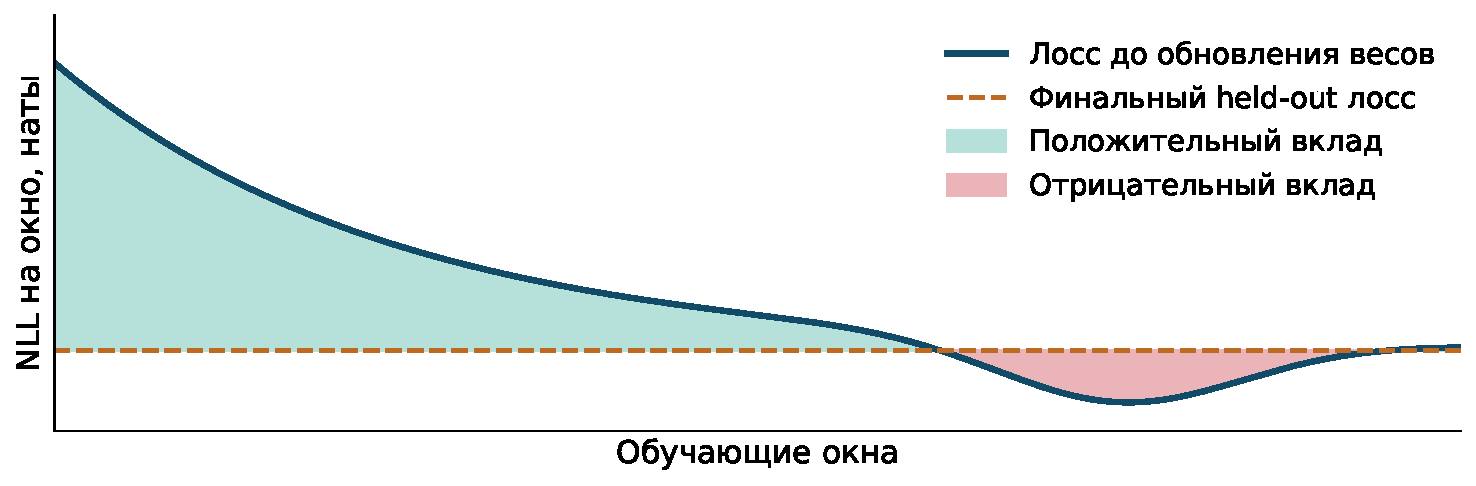
\includegraphics[width=.94\textwidth,height=35mm,keepaspectratio]{figures/area_schematic.pdf}\par
{\small \(A=\sum_i(\ell_i-\overline\ell_{\mathrm{fin}}),\qquad\widehat S=A/\ln2.\)}\par\vspace{2mm}
\smallnote{Схематическая иллюстрация, не измеренный прогон. Участки ниже baseline дают отрицательный вклад; код не обрезает площадь снизу нулём.}
\end{frame}

\begin{frame}[fragile]{Как формула реализована в коде}
\begin{lstlisting}
# PrequentialEstimator.run(...)
Trainer(model, generator, spec, config, out).run()
return self.from_run_dir(out)

# analysis.run_area(...): simplified
L_pre = losses.sum()
l_fin = heldout.mean()
A = L_pre - len(losses) * l_fin
\end{lstlisting}\vspace{1mm}
\begin{tabular}{@{}>{\raggedright\arraybackslash}p{.40\textwidth}>{\raggedright\arraybackslash}p{.56\textwidth}@{}}
\code{window_loss.f32}&Лосс каждого окна до обновления весов.\\[1mm]
\code{heldout_ema_1.f32}&Held-out лоссы конечной EMA-модели.\\[1mm]
\code{PrequentialEstimator}&Запускает обучение и переводит результат в биты.\\
\end{tabular}\vspace{2mm}
\smallnote{Исходники: \sourcefile{src/episynth/estimators/prequential.py}{estimators/prequential.py}, \sourcefile{src/episynth/analysis.py}{analysis.py}, \sourcefile{src/episynth/training.py}{training.py}.}
\end{frame}

\begin{frame}{Конфигурация маленького CPU-прогона}
\begin{columns}[T]
\column{.48\textwidth}\textbf{Данные и форма задачи}
\begin{itemize}
\item \code{waveform}, длина ряда 256;
\item контекст 128, горизонт 32;
\item размер патча 32;
\item 64 train-окна, 32 held-out;
\item батч 4: всего 16 шагов.
\end{itemize}
\column{.48\textwidth}\textbf{Модель и обучение}
\begin{itemize}
\item ширина 64, один слой;
\item 60\,994 параметра;
\item распределение Student-t;
\item CPU, fp32, init seed 0;
\item AdamW, EMA, раздельные сиды.
\end{itemize}
\end{columns}\vspace{3mm}
{\small \textbf{Связь с большими экспериментами:} те же классы, реестр и конфигурационные объекты, что и в GPU-прогонах; уменьшен вычислительный бюджет.}
\end{frame}

\begin{frame}{PoC выполнен: лоссы, held-out и оценка в битах}
\centering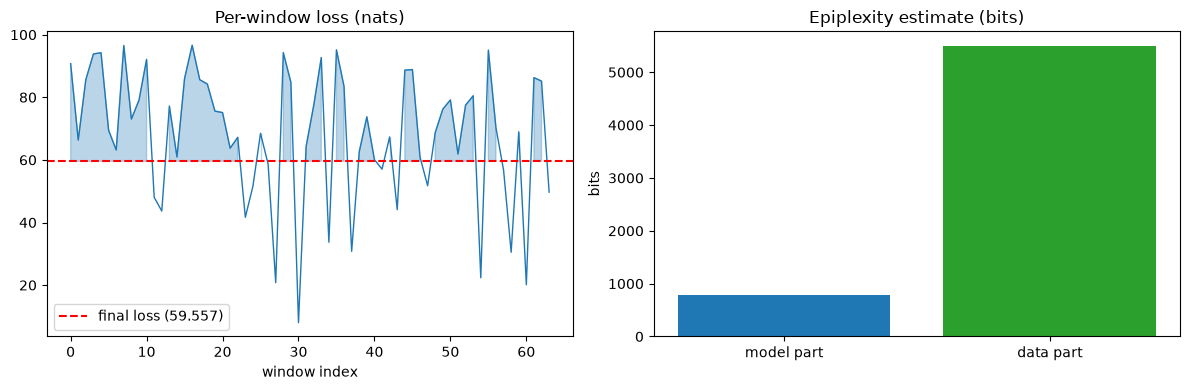
\includegraphics[width=\textwidth,height=43mm,keepaspectratio]{figures/demo_notebook.png}\vspace{2mm}
{\small\begin{tabular}{@{}ccc@{}}\textbf{Model part}&\textbf{Data part}&\textbf{Total}\\788.284 бит&5499.059 бит&6287.343 бит\end{tabular}}\par\vspace{2mm}
\smallnote{График из выполненного demo\_estimators.ipynb: 6 кодовых ячеек, ошибок выполнения нет. Заливка выделяет только участки выше baseline; численный расчёт A учитывает оба знака. Короткий прогон не доказывает сходимость оценки или корреляцию с переносом.}
\end{frame}

\begin{frame}[fragile]{Интеграция алгоритмов через один контракт}
\begin{lstlisting}
class EpiplexityEstimator(Protocol):
    name: str
    def run(
        self, model: MoiraiModule, generator: Generator,
        spec: WindowSpec, config: TrainConfig,
        out_dir: str | Path,
    ) -> dict[str, float]: ...
\end{lstlisting}\vspace{1mm}
\begin{enumerate}
\item Реализовать \code{run}: вернуть \code{model_part_bits} и \code{data_part_bits}.
\item Зарегистрировать класс: \code{@register("name")}.
\item Выбрать через \code{build("name")} или поле JSON \code{estimator}.
\end{enumerate}\vspace{1mm}
\smallnote{Prequential реализован. Requential — каркас, вызывающий NotImplementedError. В ноутбуке ConstantEstimator показывает регистрацию, а не научный алгоритм.}
\end{frame}

\begin{frame}[fragile]{Автодок и проверки реализации}
\begin{columns}[T]
\column{.47\textwidth}\textbf{Автодок Sphinx}
\begin{lstlisting}[language={}]
.. automodule:: episynth.analysis
   :members:
\end{lstlisting}
Сигнатуры, аннотации и docstrings автоматически превращаются в API-страницу.
\vspace{3mm}\href{https://intsystems.github.io/Epiplexity/api/analysis.html\#episynth.analysis.run_area}{\color{Teal}\textbf{Открыть автодок run\_area}}
\column{.49\textwidth}\textbf{Что проверяется}
\begin{itemize}
\item pytest: формулы площади, обучение, файлы и resume;
\item генерация, окна и модель;\item Ruff: стиль и импорты;
\item Sphinx: предупреждения считаются ошибками сборки.
\end{itemize}
\end{columns}\vspace{3mm}
\smallnote{Последняя полная проверка базового кода: 72 passed, 2 skipped. Пропуски требуют внешних данных GIFT-Eval и весов Moirai. Сборка docs на push/PR, публикация Pages только вручную.}
\end{frame}

\begin{frame}{Что подтверждает Proof of Concept}
\begin{enumerate}
\item \textbf{Ноутбук:} конфигурация \(\to\) \code{build("prequential")} \(\to\) прогон \(\to\) графики и биты.
\item \textbf{Код:} контракт \(\to\) PrequentialEstimator \(\to\) общий Trainer \(\to\) \code{run_area}.
\item \textbf{Документация:} сгенерированная API-страница с параметрами и результатом функции.
\end{enumerate}\vspace{2mm}
\begin{block}{Подтверждённый результат}
Базовый алгоритм встроен в библиотеку: данные проходят весь путь от генератора до сохранённых лоссов и оценки. Интерфейс позволяет подключать новые оценщики.
\end{block}\vspace{1mm}
\href{https://github.com/intsystems/Epiplexity/blob/main/experiments/demos/demo_estimators.ipynb}{\color{Teal}\small Выполненный ноутбук}\hfill\href{https://intsystems.github.io/Epiplexity/}{\color{Teal}\small Документация}\hfill\href{https://github.com/intsystems/Epiplexity/blob/main/publications/technical_report/main.pdf}{\color{Teal}\small Технический отчёт}
\end{frame}

\appendix
\begin{frame}{Приложение: неопределённость и ограничения}
\[\operatorname{SE}(\widehat S)=\frac{N}{\ln2}\operatorname{SE}(\overline\ell_{\mathrm{fin}}),\qquad\operatorname{SE}(\overline\ell_{\mathrm{fin}})=\frac{s_{\mathrm{held}}}{\sqrt m}.\]
\begin{itemize}
\item Это ошибка от конечного held-out набора при независимости окон; она не включает разброс по сидам обучения.
\item EMA и raw endpoint могут давать разные площади. Фиксируем протокол и проверяем чувствительность.
\item Для непрерывных плотностей NLL и разложение могут быть отрицательными; важны масштаб и деквантование.
\item Один прогон не решает теоретическую оптимизацию по наблюдателям: оценка привязана к архитектуре и бюджету.
\end{itemize}
\smallnote{Отрицательная знаковая площадь сама по себе не подтверждает отрицательную теоретическую эпиплексию.}
\end{frame}

\begin{frame}{Приложение: контекст больших серий}
\centering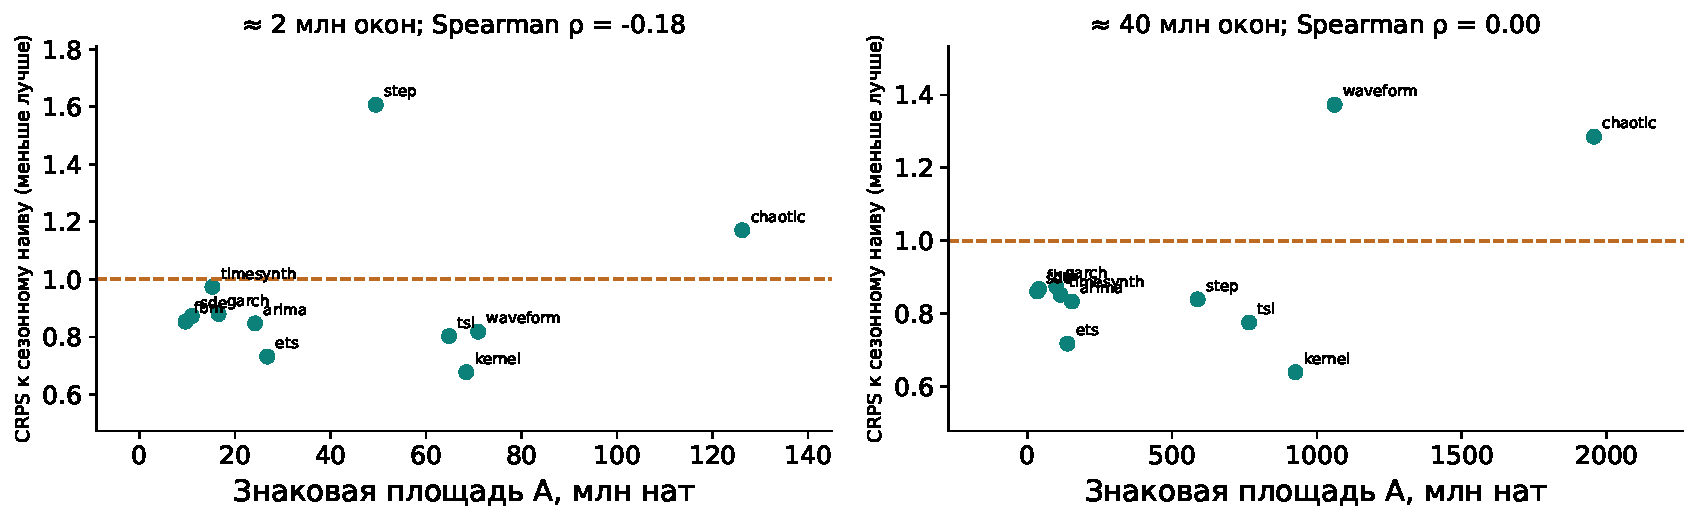
\includegraphics[width=\textwidth,height=45mm,keepaspectratio]{figures/large_series_context.pdf}
\smallnote{Источник: сохранённые CSV техотчёта, по 11 генераторов. Отдельный повтор Waveform по сиду исключён. Штриховая линия — качество сезонного наива.}
\vspace{2mm}{\small Во всех 11 семействах связь площади с агрегированным CRPS слабая: \(\rho\approx-0.18\) и \(0.00\); bootstrap-интервалы включают ноль. Это результат большого исследования, не маленького PoC.}
\end{frame}

\begin{frame}{Источники и воспроизводимость}
\small\begin{itemize}
\item Finzi et al. (2026), \textit{From Entropy to Epiplexity}. \href{https://arxiv.org/abs/2601.03220}{arXiv:2601.03220}. Теория и prequential-подход.
\item Woo et al. (2024), \textit{Unified Training of Universal Time Series Forecasting Transformers}. \href{https://arxiv.org/abs/2402.02592}{arXiv:2402.02592}. Moirai.
\item Aksu et al. (2024), \textit{GIFT-Eval}. \href{https://arxiv.org/abs/2410.10393}{arXiv:2410.10393}. Бенчмарк переноса.
\item Nagpal et al. (2026), \textit{Mix, Don't Pick}. \href{https://arxiv.org/abs/2606.09912}{arXiv:2606.09912}. Генераторы.
\end{itemize}\vspace{2mm}
\textbf{Данные:} выполненный ноутбук и CSV в \code{publications/technical_report/data/}.\par\vspace{1mm}
\textbf{Базовая ревизия:} \code{c910088}. Материалы презентации: \code{publications/slides/poc_prequential/}.\par\vspace{1mm}
\smallnote{Схема площади отделена от измеренных данных. Большие GPU-эксперименты при подготовке не перезапускались.}
\end{frame}
\end{document}
